% Created 2024-08-01 Thu 15:16
% Intended LaTeX compiler: lualatex
\documentclass[presentation,professionalfonts,smaller,aspectratio=169]{beamer}
                

% 
\makeatletter
 \@ifclassloaded{beamer}{%
  %%% save beamer's `solution' environment as `beamersolution':
  \let\beamersolution\solution
  \let\endbeamersolution\endsolution
  %%% "delete" the `solution' environment:
  \let\solution\relax
  \let\endsolution\relax
}{%
}%
\makeatother
\usepackage[utf8]{inputenc}
\usepackage[T1]{fontenc}
%\usepackage[french]{babel}
\usepackage[portuguese]{babel}

%%%% FONTS




\usepackage{xsim}
\usepackage[most]{tcolorbox}
\usepackage{amssymb}
\usepackage{fontawesome}
\newcounter{paragraph}



\DeclareExerciseEnvironmentTemplate{custom}{%
  \begin{tcolorbox}[boxrule = 0pt]
  \tcbox[on line,colback=teal,colframe=teal,coltext=white,size=small]{%
    \faBook\sffamily\bfseries\
    \XSIMmixedcase{\GetExerciseName}
    \GetExerciseProperty{counter}%
  }\quad
}{\end{tcolorbox}}


\DeclareExerciseEnvironmentTemplate{custom2}{%
  \begin{tcolorbox}[boxrule = 0pt]
  \tcbox[on line,colback=violet,colframe=violet,coltext=white,size=small]{%
    \faToggleOn\sffamily\bfseries\
    \XSIMmixedcase{\GetExerciseName}
    \GetExerciseProperty{counter}%
  }\quad
}{\end{tcolorbox}}




\DeclareExerciseType{test}{
	exercise-env = question ,
	solution-env = answer ,
	exercise-template = custom ,
	solution-template = custom2 ,
	exercise-name	= Exemplo. ,
	exercises-name = Exemplo ,
	solution-name = Solução ,
	solutions-name = Sol. ,
	exercise-heading = \textbf ,
	solution-heading = \textbf
}


\xsimsetup{
  exercise/within = section,
  exercise/the-counter =  \arabic{exercise}, 
%%solution-name = solution,  % used with headings=true
solution/print=false,
%print-collection/print=both,
}





\usepackage{colortbl}
\usepackage[tikz]{bclogo}
\usetikzlibrary{fit,patterns,shadows.blur,shapes,mindmap}
\usetikzlibrary{arrows,calc,arrows.meta,decorations.markings,shapes.symbols}
\usetikzlibrary{decorations.pathreplacing, decorations.pathmorphing,calc,arrows,positioning}
\usepackage{tikzpeople}
\usepackage{qrcode,hyperref}
\usepackage{upgreek}
%\usepackage[version=4]{mhchem}
\usepackage{tabularray}


\NewTblrTheme{fancy}{
\SetTblrStyle{caption-tag}{font=\bfseries}
\SetTblrInner[tblr,longtblr]{rowsep=2.5pt}
\DefTblrTemplate{firsthead, middlehead,lasthead}{default}{} % <---
\DefTblrTemplate{contfoot-text}{normal}{\scriptsize\textit{Continued on the next page}}
\SetTblrTemplate{contfoot-text}{normal}
}






\usepackage{chemfig,chemmacros,elements,chemformula}
\chemsetup{modules={all}}
\chemsetup[redox]{pos=top,roman=false}
\chemsetup[redox]{pos=top}
\chemsetup{redox/sep=.5em}
\chemsetup[redox]{explicit-sign=true}
\NewChemPhase\lqdd{\(\ell\)}
\NewChemPhase\gr{grafite}
\NewChemPhase\reac{reação}
\NewChemState\Enthalpy{symbol=H,superscript=,unit=\kilo\joule}%
\usepackage{siunitx}
\setchemfig{fixed length=false, atom sep=2.5em, arrow offset=6pt, scheme debug=false}%,angle increment=30}
\renewcommand*\printatom[1]{\ensuremath{\mathsf{#1}}} % This line changes the font of the atoms to sans serif
%%%% QRCODE
\usepackage{pdfpages}
\usepackage{mol2chemfig}
\usepackage{subfig,caption}
\usepackage{wrapfig}
\usepackage{enumitem}
\setitemize{label=\usebeamerfont*{itemize item}%
\usebeamercolor[fg]{itemize item}
\usebeamertemplate {itemize item}}
\usepackage{array} % ajust colunm table
\usepackage{cancel}
\usepackage[controls]{animate}
\renewcommand{\CancelColor}{\color{red}}

%%%%%%%%%%%%%%%%%%% CONFIG TCOLORBOX 

\newtcolorbox{mybox}[2][]{boxsep=0.5em,left=0.5em,
colback=blue!5!white, colframe=blue!75!black,
fonttitle=\bfseries\sffamily,
colbacktitle=blue!85!red!60,enhanced,
attach boxed title to top left={yshift=-3mm,xshift=5mm},
title=#2,#1}

\newtcolorbox{myrule}[2][]{boxsep=0.5em,left=0.5em,
colback=green!5!white, colframe=blue!75!black,
fonttitle=\bfseries\sffamily,
colbacktitle=blue!85!red!60,enhanced,
attach boxed title to top left={yshift=-3mm,xshift=5mm},
title=#2,#1}


\newtcolorbox{myex}[2][]{boxsep=0.5em,left=0.5em,
  colback=yellow!5!white, colframe=blue!75!black, 
  fonttitle=\bfseries\sffamily,
  colbacktitle=blue!85!red!60,enhanced,
  attach boxed title to top left={yshift=-3mm,xshift=5mm},
  title=#2,#1}


 \definecolor{col1}{HTML}{FF7878}
 \definecolor{col2}{HTML}{51B5F8}
 \definecolor{col3}{HTML}{68E1AA}
 \definecolor{col4}{HTML}{B869EA}
 \definecolor{col5}{HTML}{FF5500}
 \definecolor{col6}{HTML}{FFF8E7}
 \definecolor{col7}{HTML}{FF9966}
 \definecolor{col8}{HTML}{9400D3}



\definesubmol\nobond{-[,0.2,,,draw=none]\scriptstyle\color{blue}}
\newcommand{\re}{\hspace{-1cm}}
\newcommand{\af}{\hspace{2cm}}

%%%% Config X sim for BEAMER
\makeatletter
\@ifclassloaded{beamer}{%
%%% save beamer's `solution' environment as `beamersolution':
\let\beamersolution\solution
\let\endbeamersolution\endsolution
%%% "delete" the `solution' environment:
\let\solution\relax
\let\endsolution\relax
}{%
}%
\makeatother
\usepackage[utf8]{inputenc}
\usepackage[T1]{fontenc}
%\usepackage[portuguese, ]{babel}
%%%% FONTS
%%% XSIM CONFIG BEAMER
\usepackage{xsim}
\usepackage[most]{tcolorbox}
\usepackage{amssymb}
\usepackage{fontawesome}
\usepackage{tasks}
\newcounter{paragraph}
\usepackage[dvipsnames,svgnames]{xcolor}
\usepackage{annotate-equations}
%%% BOX EXERCISE BEAMER
\DeclareExerciseEnvironmentTemplate{custom}{%
\begin{tcolorbox}[boxrule = 0pt]
\tcbox[on line,colback=teal,colframe=teal,coltext=white,size=small]{%
\faBook\sffamily\bfseries\
\XSIMmixedcase{\GetExerciseName}
\GetExerciseProperty{counter}%
}\quad
}{\end{tcolorbox}}
%% == CUSTOM BOX BEAMER
\DeclareExerciseEnvironmentTemplate{custom2}{%
\begin{tcolorbox}[boxrule = 0pt]
\tcbox[on line,colback=violet,colframe=violet,coltext=white,size=small]{%
\faToggleOn\sffamily\bfseries\
\XSIMmixedcase{\GetExerciseName}
\GetExerciseProperty{counter}%
}\quad
}{\end{tcolorbox}}
\DeclareExerciseType{test}{
exercise-env = question ,
solution-env = answer ,
exercise-template = custom ,
solution-template = custom2 ,
exercise-name = Exemplo. ,
exercises-name = Exemplo ,
solution-name = Solução ,
solutions-name = Sol. ,
exercise-heading = \textbf ,
solution-heading = \textbf
}
\xsimsetup{
exercise/within = section,
exercise/the-counter =  \arabic{exercise},
%%solution-name = solution,  % used with headings=true
solution/print=false,
print-collection/print=both,
}
\NewTasksEnvironment[label = (\emph{\alph*}),
label-width = 12pt]{choice}[\choice]
\usepackage{colortbl}
\usepackage[tikz]{bclogo}
\usetikzlibrary{fit,patterns,shadows.blur,shapes,mindmap}
\usetikzlibrary{arrows,arrows.meta,decorations.markings,shapes.symbols}
\usetikzlibrary{decorations.pathreplacing, decorations.pathmorphing,calc,arrows,positioning}
\usepackage{tikzpeople}
\usepackage{qrcode,hyperref}
\usepackage{upgreek}
%\usepackage[version=4]{mhchem}
\usepackage{tabularray}
%%% CUSTOM TABLE
\NewTblrTheme{fancy}{
\SetTblrStyle{caption-tag}{font=\bfseries,red2}
\SetTblrInner[tblr,longtblr]{rowsep=2.5pt}
\DefTblrTemplate{firsthead, middlehead,lasthead}{default}{} % <---
\DefTblrTemplate{contfoot-text}{normal}{\scriptsize\textit{Continua ...}}
\SetTblrTemplate{contfoot-text}{normal}
}
%% ==== CHEMMACROS E CHEMFIG CONFIG
\usepackage{chemfig,chemmacros,elements,chemformula}
\chemsetup{modules={all}}
\chemsetup[redox]{pos=top,roman=false}
\chemsetup[redox]{pos=top}
\chemsetup{redox/sep=.5em}
\chemsetup[redox]{explicit-sign=true} %%% reaction redox
%% == CUSTOM PHASES IN CHEMMACROS
\NewChemPhase\lqdd{\(\ell\)}
\NewChemPhase\gr{grafite}
\NewChemPhase\reac{reação}
\NewChemState\Enthalpy{symbol=H,superscript=,unit=\kilo\joule}%
\usepackage{siunitx}
\setchemfig{fixed length=false, atom sep=2.5em, arrow offset=6pt, scheme debug=false}
%% == NUMEROS PARA FORMULES
\renewcommand*\printatom[1]{\ensuremath{\mathsf{#1}}} % This line changes the font of the atoms to sans serif
%%% INCLUDE PAGES PDFs
\usepackage{pdfpages}
\usepackage{mol2chemfig}
\usepackage{subfig,caption}
\usepackage{wrapfig}
\usepackage{enumitem}
\setitemize{label=\usebeamerfont*{itemize item}%
\usebeamercolor[fg]{itemize item}
\usebeamertemplate {itemize item}}
\usepackage{array} % ajust colunm table
\usepackage{cancel}
\usepackage[controls]{animate}
\renewcommand{\CancelColor}{\color{red}}
%%%%%%%%%%%%%%%%%%% CONFIG TCOLORBOX
\newtcolorbox{mybox}[2][]{boxsep=0.5em,left=0.5em,
colback=blue!5!white, colframe=blue!75!black,
fonttitle=\bfseries\sffamily,
colbacktitle=blue!85!red!60,enhanced,
attach boxed title to top left={yshift=-3mm,xshift=5mm},
title=#2,#1}
\newtcolorbox{myrule}[2][]{boxsep=0.5em,left=0.5em,
colback=green!5!white, colframe=blue!75!black,
fonttitle=\bfseries\sffamily,
colbacktitle=blue!85!red!60,enhanced,
attach boxed title to top left={yshift=-3mm,xshift=5mm},
title=#2,#1}
\newtcolorbox{myex}[2][]{boxsep=0.5em,left=0.5em,
colback=yellow!5!white, colframe=blue!75!black,
fonttitle=\bfseries\sffamily,
colbacktitle=blue!85!red!60,enhanced,
attach boxed title to top left={yshift=-3mm,xshift=5mm},
title=#2,#1}
\definecolor{col1}{HTML}{FF7878}
\definecolor{col2}{HTML}{51B5F8}
\definecolor{col3}{HTML}{68E1AA}
\definecolor{col4}{HTML}{B869EA}
\definecolor{col5}{HTML}{FF5500}
\definecolor{col6}{HTML}{FFF8E7}
\definecolor{col7}{HTML}{FF9966}
\definecolor{col8}{HTML}{9400D3}
\definesubmol\nobond{-[,0.2,,,draw=none]\scriptstyle\color{blue}}
\newcommand{\re}{\hspace{-1cm}}
\newcommand{\af}{\hspace{2cm}}
\date{}
%\usetheme{minflat}
\DeclareExerciseCollection{Hidro}
\usetheme{minflat}
\author{Fábio Lima}
\date{}
\title{Hidrocarbonetos}
\hypersetup{
 pdfauthor={Fábio Lima},
 pdftitle={Hidrocarbonetos},
 pdfkeywords={},
 pdfsubject={},
 pdfcreator={Emacs 29.4 (Org mode 9.6.15)}, 
 pdflang={En Portuguese}}
\begin{document}

\maketitle
\begin{frame}{Sumário}
\tableofcontents
\end{frame}




\section{Hidrocarbonetos}
\label{sec:org001990b}
\begin{frame}[label={sec:orga7a5ded}]{Hidrocarbonetos}

\begin{tikzpicture}
%\tikzstyle{every node}=[fill=red!30,rounded corners]
%\tikzstyle{edge from parent}=[red,thick,draw]
[main/.style={fill=red!30,rounded corners,font={\bfseries\small}},
main1/.style={fill=green!30,rounded corners,font={\bfseries\small}, align=center, minimum size=10mm, text width=15mm},
main2/.style={fill=violet!30,rounded corners,font={\bfseries\small}, align=center},
%edge from parent ./style={red,-o,thick,draw},
level distance=2cm,
level 1/.style={sibling distance=4.cm},
level 2/.style={sibling distance=2.5cm,level distance=1.5cm},
level 3/.style={sibling distance=4.5cm,level distance=1.5cm,font={\bfseries\tiny}}, edge from parent fork down,
grand/.style={grow=down,xshift=1em,anchor=west, edge from parent path={(\tikzparentnode.south) |- (\tikzchildnode.west)}},
 first/.style={level distance=4ex},
 second/.style={level distance=8ex},
 third/.style={level distance=12ex},
 four/.style={level distance=16ex},
 ]
\node [main]{Hidrocarbonetos}
    child {node[main1] {Cadeia Aberta} 
    	child [grand,first]{node [main2]{Alcanos}}
    	child [grand,second] {node [main2]{Alcenos}}
    	child [grand,third]{node [main2]{Alcinos}}
    	child [grand,four] {node [main2]{Alcadienos}}
    }
    child {node[main1] {Cadeia Aromática}	
    	child {node[main2] {Aromáticos}}
    }
   %%%%%
    child {node[main1]{Cadeia Fechada}
      child {node[main2] {Ciclanos}}
      child {node[main2] {Ciclenos}}
    };
\end{tikzpicture}
\begin{tikzpicture}
		\begin{scope}[yshift=5cm, xshift=-2cm]
		\node[draw=none,text width=10cm, minimum size=10mm, font=\small] (-5,5) {$\bullet$ São compostos orgânicos formados exclusivamente por átomos de C e de H.
			};
		\end{scope}
		\begin{scope}[yshift=5cm,xshift=-8cm]
		\coordinate (dv) at (0,0);
		\coordinate (base) at (25pt,0pt);
		\coordinate (height) at (0pt,25pt);
		\coordinate (diag) at ($(base)+(height)$);
		\fill[rounded corners=2pt, violet] ($(dv)-.5*(diag)$) rectangle +(diag); 
		\node[white] at (dv) {\sffamily\huge C};
		\node[white, inner sep=2pt] (dvtext) at ($(dv)-.5*(height)$) [anchor=south] {\sffamily\tiny Carbono};
		\node[white, inner sep=2pt] (dvnum) at ($(dv)+.5*(height)-.5*(base)$) [anchor=north west] {\sffamily\tiny 6};
		\end{scope}
		\end{tikzpicture}
\end{frame}



\begin{frame}[label={sec:org42c9a8f}]{Hidrocarbonetos}
\begin{itemize}
\item Podem ser obtidos a partir da destilação fracionada do petróleo. Esquema de uma torre de fracionamento.
\end{itemize}

\begin{figure}[htbp]
\centering
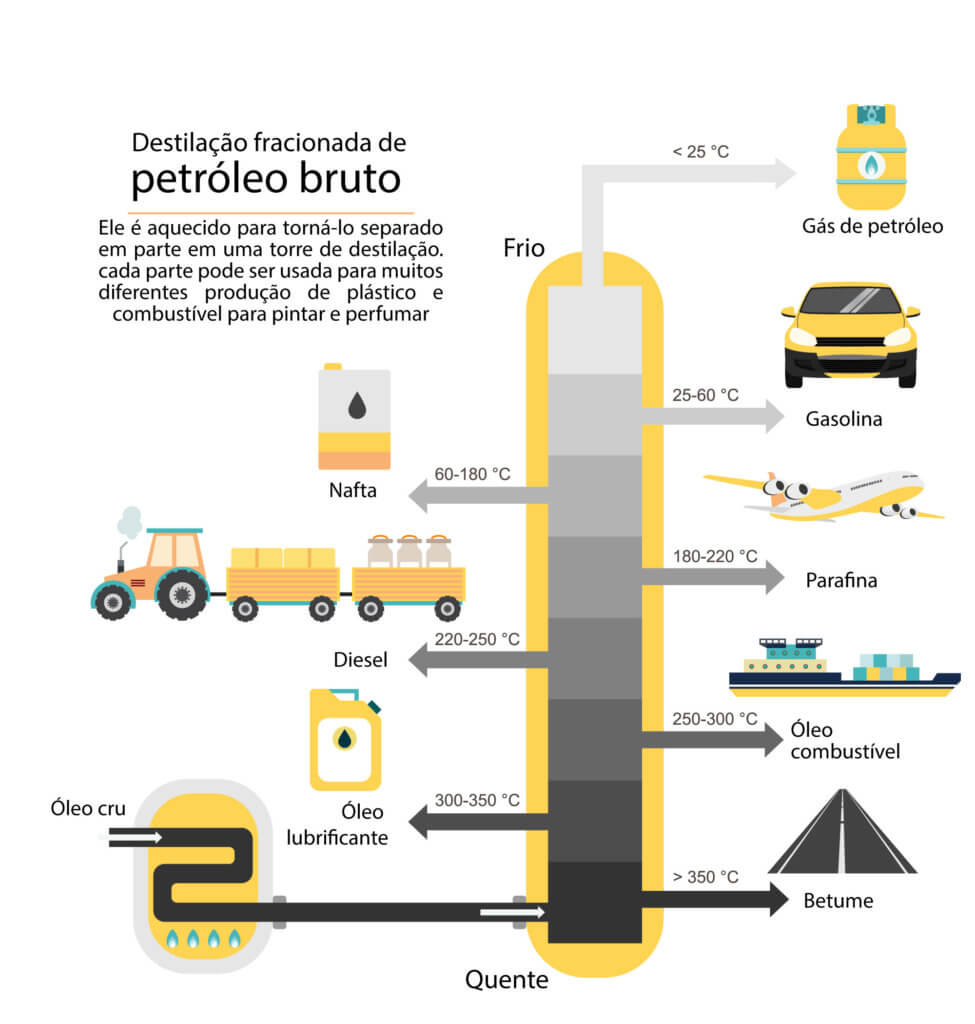
\includegraphics[width=0.4\textwidth]{QO/Hidrocarbonetos/torre.jpg}
\caption{\label{fig:org80a15d9}Esquema de uma torre de fracionamento.}
\end{figure}
\end{frame}

\begin{frame}[label={sec:org38af3a7}]{Frações Típicas do Petróleo}
%		{\centering \small
			\begin{talltblr}[
				theme= fancy,
				caption={Composição do Petróleo},
				]{
					colspec = {lccc}, colsep = 2mm, hlines = {2pt, white},
					row{odd} = {brown8}, row{even} = {gray8},
					row{1} = {2em,azure2,fg=white,font=\bfseries},
					%row{2-Z} = {3em,font=\large},
				}
				%	\hline
				Fração   &  {Temperatura de Ebulição (°C)}   &  {Composição \\  aproximada}  &  Usos \\
				%	\hline
				Gás residual & - &  \ch{C1-C2} & gás combustível\\
				\hline
				{Gás liquefeito \\ de petróleo - GLP} & Até 40 &  \ch{C3-C4}  & gás para uso doméstico e indrustrial\\
				\hline
				Gasolina & 40-175 & \ch{C5-C10} & automóveis, solvente\\
				\hline
				Querosene & 175-235 & \ch{C11-C12} & iluminação, combustível aviões\\
				\hline
				Gasoléo leve & 235-305 & \ch{C13-C17} & diesel, fornos\\
				\hline
				Gasoléo pesado & 305-400 & \ch{C18-C25} & combustível, lubrificantes\\
				\hline
				Lubrificantes & 400-510 & \ch{C26-C38} & óleos librificantes\\
				\hline
				Resíduo & Acima de 510 & \ch{C38-} & asfalto, piche, impermeabilizantes \\
				\hline
			\end{talltblr}
%		}
\end{frame}

\section{Classificação}
\label{sec:orgb72d7ff}

\begin{frame}[label={sec:orge34f607}]{Grupos}
\begin{itemize}
\item Os nomes \alert{alcanos}, \alert{alcenos}, \alert{alcinos}, \alert{alcadienos}, \alert{ciclanos}, \alert{ciclenos} e \alert{aromáticos} designam grupos aos quais os hidrocarbonetos pertencem.
\end{itemize}

\vspace{0.1cm}
\begin{tikzpicture}
\tikzset{grow'=right,level distance=32mm}
\tikzset{edge from parent/.style={draw,edge from parent fork right,red},-o,thick}
\tikzset{level 1/.style={sibling distance=3.2cm}}
\tikzset{level 2/.style={sibling distance=1.0cm,level distance=2.5cm},}
\tikzset{main/.style={draw,rounded corners,font={\bfseries\small}, align=center, text width=17mm}}
\tikzset{main1/.style={font={\bfseries\small}, align=center}}
\tikzset{every tikzmarknode/.append style={inner sep=3pt,rounded
corners}}
%\begin{scope}[frontier/.style={distance from root=5mm}]
\node[main] {Cadeia}
	child {node[main] {Alifática (aberta)}
		child {node[main1] {Alc\tikzmarknode[fill=red!30]{Red1}{an}o}}
		child {node[main1]{Alc\tikzmarknode[fill=green!30]{Green1}{en}o}}
		child {node[main1]{Alc\tikzmarknode[fill=blue!30]{Blue1}{in}o}}
		child {node[main1]{Alca\tikzmarknode[fill=yellow!30]{Yellow1}{dien}o}}
		}
	child {node [main] {Cíclica (fechada)}	
		child [main1]{node {Cicl\tikzmarknode[fill=Teal!50]{Teal1}{an}o}}
		child [main1]{node {Cicl\tikzmarknode[fill=DarkOrchid!50]{DarkOrchid1}{en}o}}
};
%\end{scope}
%%%%% LINHAS 
\node[main1] at (9.5,3.1){\tikzmarknode[fill=red!30]{Red2}{an} indica apenas uma ligação simples};
\node[main1] at (9.5,2.1){\tikzmarknode[fill=green!30]{Green2}{en} indica apenas uma ligação dupla};
\node[main1] at (9.5,1.1){\tikzmarknode[fill=blue!30]{Blue2}{in} indica apenas uma ligação tripla};
\node[main1] at (9.2,0.1){\tikzmarknode[fill=yellow!30]{Yellow2}{dien} indica duas ligações duplas};
\node[main1] at (9.5,-1.1){\tikzmarknode[fill=Teal!50]{Teal2}{an} indica uma  ligação simples};
\node[main1] at (9.3,-2.1){\tikzmarknode[fill=DarkOrchid!50]{DarkOrchid2}{en} indica uma ligação dupla};
%%%%% SETA DE LIGACAO

\end{tikzpicture}
\annotatetwo[->]{below}{Red1}{Red2}{}
\annotatetwo[->]{below}{Green1}{Green2}{}
\annotatetwo[->]{below}{Blue1}{Blue2}{}
\annotatetwo[->]{below}{Yellow1}{Yellow2}{}
\annotatetwo[->]{below}{Teal1}{Teal2}{}
\annotatetwo[->]{below}{DarkOrchid1}{DarkOrchid2}{}
\end{frame}



\begin{frame}[allowframebreaks]{Subdivisões dos hidrocarbonetos}
	
	\begin{longtblr}[
		theme = fancy,
		caption = {Subdivisões importantes dos hidrocarbonetos},
		entry = {Short Caption},
		label = {tblr:test},
		]{
		colspec = {cccc}, colsep = 2mm, hlines = {2pt, white},
		rowsep = 3.5pt, %% space line 
		row{1} = {2em,azure2,fg=white,font=\bfseries\sffamily},
		 }
\hline
Subgrupo  & Característica  & Exemplos  & Fórmula geral \\
\hline
{Alcanos\\ ou parafinas} & {Cadeia aberta \\ Ligações simples} & {\chemfig{H_3C-CH_2-CH_3} \\  \chemfig{H_3C-C([:90]-CH_3)([:-90]-CH_3)-CH([:-90]-CH_3)-CH_3}} &  \(\mathrm{C_nH_{2n+2}}\) \\
 \hline
 {Alcenos,  \\ alquenos \\ ou olefinas} & {Cadeia aberta com \\ 1 ligação dupla} & {\chemfig{H_2C=CH-CH_2-CH_3} \\ \chemfig{H_3C-C([:90]-CH_3)=CH-CH_3}} & \(\mathrm{C_nH_{2n}}\)\\
 \hline \pagebreak
 {Alcinos \\ ou alquinos} & {Cadeia aberta \\ 1 ligação tripla} & {\chemfig{HC~C-CH_3} \\ \chemfig{H_3C-C([:90]-CH_3)([:-90]-CH_3)-C~C-CH_3}} & \(\mathrm{ C_nH_{2n-2}}\)\\ 
 \hline
 {Alcadienos \\ ou dienos} & {Cadeia aberta \\ 2 ligações duplas} & {\chemfig{H_2C=C=CH_2} \\[1pt] \chemfig{H_2C=CH-CH=CH_2}} & \(\mathrm{C_nH_{2n-2}}\)\\
 \hline \pagebreak
 Ciclanos & {Cadeia fechada \\ Ligações simples} & {\chemfig{*6(------)}} & \(\mathrm{C_nH_{2n}}\)\\
 \hline 
 Ciclenos & { Cadeia fechada \\  uma ligação dupla} & {  \chemfig{*6(-----=)}} & \(\mathrm{C_nH_{2n-2}}\)\\
 \hline \pagebreak
 Aromáticos & Contêm anel benzênico & {\chemfig{**6(-----(-CH_3)-)} \\   \chemfig{*6(-=-(*6(-=-=---))=-=)}} & \(\mathrm{C_nH_{2n-6}}\)\\
 \hline 
\end{longtblr}
\end{frame}



\section{Nomenclatura}
\label{sec:org0f3f6c3}
\begin{frame}[allowframebreaks]{Nomenclatura dos compostos orgânicos}
\begin{myrule}{Regra}
\begin{itemize}
\item A nomenclatura de compostos orgânicos segue as regras elaboradas pela IUPAC.

\item De acordo com as regras da IUPAC, o nome de um composto orgânico é formado pela união de três fragmentos: \alert{prefixo + infixo + sufixo}.
\end{itemize}

\end{myrule}
\end{frame}

\begin{frame}[label={sec:org4435ed1}]{Nomenclatura dos compostos orgânicos}
\begin{itemize}
\item O prefixo, a parte inicial, indica o número de átomos de carbono presentes na molécula.
\end{itemize}


\begin{longtblr}[theme=fancy,
    caption = {Grupos substituintes orgânicos formados por carbono e hidrogênio},]
    {
        colspec = {c c c c }, colsep = 2mm, hlines = {2pt, white},
        %row{odd} = {azure8}, row{even} = {gray8},
        row{1} = {1.5em,azure2,fg=white,font=\bfseries\sffamily},
        }
\hline
Prefixo  &  Número de carbonos  &  Prefixo  & Número de carbonos \\[0pt]
\hline
met & 1 & undec & 11\\[0pt]
et & 2 & dodec & 12\\[0pt]
prop & 3 & tridec & 13\\[0pt]
but & 4 & tretadec & 14\\[0pt]
pent & 5 & pentadec & 15\\[0pt]
hex & 6 & hexadec & 16\\[0pt]
hept & 7 & hepdec & 17\\[0pt]
oct & 8 & octadec & 18\\[0pt]
non & 9 & nonadec & 19\\[0pt]
dec & 10 & icosa & 20\\[0pt]
\hline
\end{longtblr}
\end{frame}

\begin{frame}[label={sec:orge2e3e67}]{Nomenclatura dos compostos orgânicos}
\begin{itemize}
\item O \alert{infixo} indica o tipo de ligação química entre os átomos de carbono.
\end{itemize}


\begin{talltblr}[theme=fancy,
caption = {Infixos para a nomenclatura orgânica},
entry = {Short Caption},
label = {tblr:tall},
%note{a} = {It is the first footnote.},
%note{$\dag$} = {It is the second long long long long long long footnote.},
]{
colspec = {XX}, colsep = 2mm, hlines = {2pt, white},
row{1} = {1.5em,azure2,fg=white,font=\bfseries\sffamily},
}
\hline 
Infixo  &  Tipo de Ligação \\
\hline
an & simples\\
en & dupla\\
in & tripla\\
\hline
\end{talltblr}
\end{frame}



\begin{frame}[label={sec:org4cb5a80}]{Nomenclatura dos compostos orgânicos}
\begin{itemize}
\item O \alert{sufixo}, a parte final, indica a \alert{classe funcional do composto}.
\end{itemize}

\begin{talltblr}[theme=fancy,
caption = {Sufixo para a nomenclatura orgânica},
entry = {Short Caption},
label = {tblr:tall},
%note{a} = {It is the first footnote.},
%note{$\dag$} = {It is the second long long long long long long footnote.},
]{
colspec = {XX}, colsep = 2mm, hlines = {2pt, white},
row{1} = {1.5em,azure2,fg=white,font=\bfseries\sffamily},
}
\hline 
Sufixo  &  Classe funcional \\
\hline
o & hidrocarbonet \alert{o}\\
ol & álco \alert{ol}\\
al & \alert{al} deído\\
ona & cet \alert{ona}\\
óico & ácido carboxíl \alert{ico}\\
\hline
\end{talltblr}
\end{frame}


\section{Exercícios}
\label{sec:org6944560}
\begin{frame}[allowframebreaks]{Exemplos}
\begin{question}
(\alert{FATEC}) O hidrocarboneto que apresenta a menor quantidade de átomos de H por molécula é:

\begin{choice}(5)
\choice metano.
\choice etano.
\choice eteno.
\choice etino.
\choice propino.
\end{choice}
\end{question}
\only<1>
\begin{answer}[print=true]
(\alert{FATEC}) O hidrocarboneto que apresenta a menor quantidade de átomos de H por molécula é:

\begin{choice}(5)
\choice metano.
\choice etano.
\choice eteno.
\choice \alert{etino}.
\choice propino.
\end{choice}

Os compostos etano e propano são hidrocarbonetos da classe dos alcanos. Portanto apresentam o número de hidrogênios maior que o número de carbonos, pois sua fórmula geral é  \ch{C_nH_{2n+2}}.

O eteno apresenta ligação dupla entre os dois carbonos, pois é um alceno de fórmula geral  \ch{C_nH_{2n}}.

Etino e propino são alcinos, pois possuem uma tripla ligação entre os carbonos. Entretanto, o propino possui um maior número de hidrogênios, já que possui um carbono a mais na cadeia. A fórmula geral de um alcino é  \ch{C_nH_{2n-2}}.

Portanto, o \alert{etino} possui apenas dois átomos de carbono (\ch{C2H2}), sendo o alcino mais simples
\end{answer}
\end{frame}



\begin{frame}[label={sec:org89b7b70}]{Fim da Aula}
\begin{tikzpicture}
\node[graduate,sword, minimum size=1cm]{ \bfseries Bons Estudos !!!!};
\end{tikzpicture}
\begin{center}
\begin{tabular}{ccc}
Download Aula & & Lista de Exercícios \\
 \qrcode[height=2in]{https://mark.nl.tab.digital/s/2qnZtdzAjYynDWw} & & \qrcode[height=2in]{https://mark.nl.tab.digital/s/eC3yxDocrjxEr4N}\\
 \end{tabular}
 \end{center}
\end{frame}
\end{document}
